\documentclass{article}

%语言页面以及字体设置
\usepackage{ctex}
\usepackage{a4}
\usepackage{indentfirst}
\setlength{\parindent}{2em}
\usepackage{xeCJK}
\usepackage{fontsize}
\usepackage{subfigure}
\usepackage{subcaption}

%其他宏包
\usepackage{amsmath}
\usepackage{graphicx}
\usepackage[a4paper, left=2.5cm, right=2.5cm, top=2.5cm, bottom=2.5cm]{geometry}
\usepackage{appendix}
\usepackage{listings,matlab-prettifier}


\lstset{style=Matlab-editor,numbers = left,frame = single,}

\title{\HUGEr \bf \kaishu 非采暖房间温度估算}
\author{葛逸凡 \quad 3210103331}
\date{\today}

\begin{document}

\maketitle

\tableofcontents

\newpage

\section{问题描述以及模型设置}

我们住在大楼里,冬天有人开暖气、空调、地暖等取暖,夏天有人开空调制冷清凉。
本文根据传热学知识,考虑以下方面分析邻居们制冷、制热对所处房间温度的影响,并利用代码和可视化方法分析房间温度的变化情况。

\subsection{初始条件以及边界条件}
初始条件:初始房间温度与环境温度相同,冬天为10摄氏度,夏天为35摄氏度。

边界条件:在分析隔壁房间温度时考虑墙体的隔热效果,在分析所处房间的温度时考虑墙壁的导热效果。

\subsection{房间简化模型}
本文为了计算方便,将房间简化为$3m\times3m\times3m$的正方体,同时设定房间墙壁厚度为$0.2m$,具体布局如下图所示:

\begin{figure}[h]
    \centering
    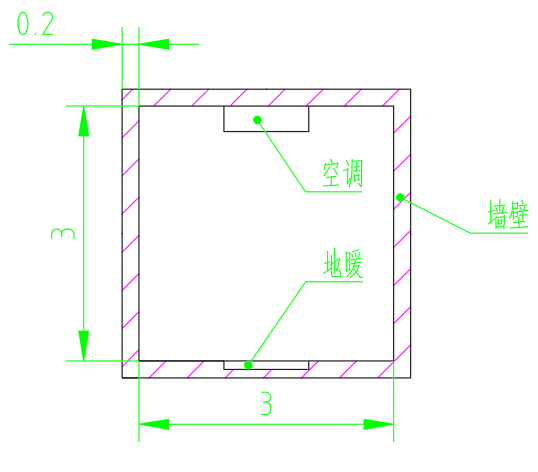
\includegraphics[scale = 0.5]{figures/房间模型.png}
    \caption{房间布局简化模型}
    \label{fig:Room}
\end{figure}

其中空调设置为扫风模式,简化为一个恒温热源以匀速在空间内上下移动,形成第一类边界条件,热源温度即为空调设定温度。

地暖简化为热流大小固定的热源,忽略其厚度,与墙壁一起组成第二类边界条件。

\subsection{传热过程}
因为同时考虑四面墙壁的导热过程以及空调和地暖的工作,其中空调设置为随时间变化的扫风模式,该传热问题为二维非稳态传热过程,使用有限差分法进行求解。




\section{有限差分法求解非稳态热传导方程}

\subsection{公式推导}

对于二维非稳态传热过程,不考虑内热源有:
\begin{equation}\label{二维非稳态传热}
    \frac{\partial T}{\partial t} = a^2(\frac{\partial^2 T}{\partial x^2}+\frac{\partial^2 T}{\partial y^2})
\end{equation}

考虑二阶导数$\partial^2 T/\partial x^2$,该导数在$(m,n)$处的值可以近似写为:
\begin{equation}\label{x非稳态传热}
    \frac{\partial^2 T}{\partial x^2}\big|_{m,n} \approx \frac{\partial T/\partial x\big|_{m+\frac{1}{2},n}-\partial T/\partial x\big|_{m-\frac{1}{2},n}}{\Delta x}
\end{equation}

其中:
\begin{equation}
    \frac{\partial T}{\partial x}\big|_{m+\frac{1}{2},n} \approx \frac{T_{m+1,n}-T_{m,n}}{\Delta x}
\end{equation}

\begin{equation}
    \frac{\partial T}{\partial x}\big|_{m-\frac{1}{2},n} \approx \frac{T_{m,n}-T_{m-1,n}}{\Delta x}
\end{equation}

因此\eqref{x非稳态传热}可以写作:
\begin{equation}\label{x方向二阶导数离散化}
    \frac{\partial^2 T}{\partial x^2}\big|_{m,n} \approx \frac{T_{m+1,n}+T_{m-1,n}-2T_{m,n}}{(\Delta x)^2}
\end{equation}

同理,对于二阶导数$\partial^2 T/\partial y^2$也有:
\begin{equation}\label{y方向二阶导数离散化}
    \frac{\partial^2 T}{\partial y^2}\big|_{m,n} \approx \frac{T_{m,n+1}+T_{m,n-1}-2T_{m,n}}{(\Delta y)^2}
\end{equation}

考虑一阶导数$\partial T/\partial t$,该导数可以近似写成:
\begin{equation}
    \frac{\partial T}{\partial t} \approx \frac{T^{N+1} - T^N}{\Delta t}
\end{equation}

式中$N$表示当前时刻,有$t =(N-1)\Delta t$.\eqref{二维非稳态传热}可以写作:
\begin{equation}
    \begin{aligned}
        T^{N+1} &= \frac{\partial T}{\partial t} \cdot \Delta t + T^N \\
                &= T^N + a^2(\frac{\partial^2 T}{\partial x^2}+\frac{\partial^2 T}{\partial y^2})\Delta t\\
                &= T^N +a^2(\frac{T_{m+1.n}+T_{m-1,n}-2T_{m,n}}{(\Delta x)^2}+\frac{T_{m.n+1}+T_{m,n-1}-2T_{m,n}}{(\Delta y)^2})\Delta t
    \end{aligned}
\end{equation}

为了方便代码的编写,将公式推广到矩阵。设$x$方向步长为$dx$,$y$方向步长为$dy$,时间步长为$dt$。$x=(i-1)dx,y=(j-1)dy,t=(N-1)dt,N_x=L_x/dx,N_y=L_y/dy$,.则有温度分布矩阵:
\begin{equation}
\boldsymbol{T^N} =
    \begin{pmatrix}
        T_{11}^N        & \cdots & T_{1  N_y+1}^N   \\
        \vdots          &        & \vdots           \\
        T_{N_x+1 1}^N   & \cdots & T_{N_x+1 N_y+1}^N\\
    \end{pmatrix}
\end{equation}

\eqref{x方向二阶导数离散化}可以写作:
\begin{equation}
    \frac{\partial^2 \boldsymbol{T^N}}{\partial x^2} =\frac{1}{dx^2}\boldsymbol{A}\boldsymbol{T^N}
\end{equation}

其中$\boldsymbol{A}$为系数矩阵,
\begin{equation}
\boldsymbol{A} =
    \begin{pmatrix}
        -2 &   1 & 0  & \cdots  \\
        1  &  -2 & 1  &  \\
        0  &   1 & \ddots &        & \vdots \\
        \vdots \\
    \end{pmatrix}
\end{equation}

\eqref{y方向二阶导数离散化}写作:
\begin{equation}
    \frac{\partial^2 \boldsymbol{T^N}}{\partial y^2} = (\frac{1}{dy^2}\boldsymbol{A}\boldsymbol{T^N}^T)^T = \frac{1}{dy^2}\boldsymbol{T^N}\boldsymbol{A}
\end{equation}

得到:
\begin{equation}\label{final equation}
    \boldsymbol{T^{N+1} = \boldsymbol{T^N}} + a^2(\frac{1}{dx^2}\boldsymbol{A}\boldsymbol{T^N}+\frac{1}{dy^2}\boldsymbol{T^N}\boldsymbol{A}) dt  
\end{equation}

在写代码时,由于$dt$取的数值极小(0.001s),因此可以将$\boldsymbol{T^{N+1}}$用$\boldsymbol{T^N}$代替,减少复杂度。

\subsection{边界条件}

主要考虑第二类边界条件:
\begin{equation}
    \frac{\partial T}{\partial x} = -q''_s/k
\end{equation}
有:
\begin{equation}
    T_{x+dx} = T_x -\frac{q''_s}{k}dx
\end{equation}


\section{隔壁房间温度估算}

对于隔壁房间,分别分析开暖气、地暖和空调的情况。同时考虑墙壁的导热效果对房间温度的影响,简化为;
\begin{equation}
    \begin{aligned}
    q''_s &= -k_{wall}\frac{T_s - T_{\infty}}{L_{wall}} \\
    T_{x+dx} &= T_x +  \frac{T_s - T_{\infty}}{L_{wall}}dx
    \end{aligned}
\end{equation}
    


将隔壁房间墙壁处的平均温度作为所处房间的边界条件。

\subsection{暖气}

暖气简化为一个以匀速在空间内上下移动的恒温热源。当外界温度及室内初始温度为10℃,室内设定温度为25℃时,通过\eqref{final equation}可以得出随时间变化的房间温度分布。

房间内某几个时刻的温度分布如下图所示:
\\
\begin{figure}[h]
    \centering
    \subfigure[空调刚开启时]{
    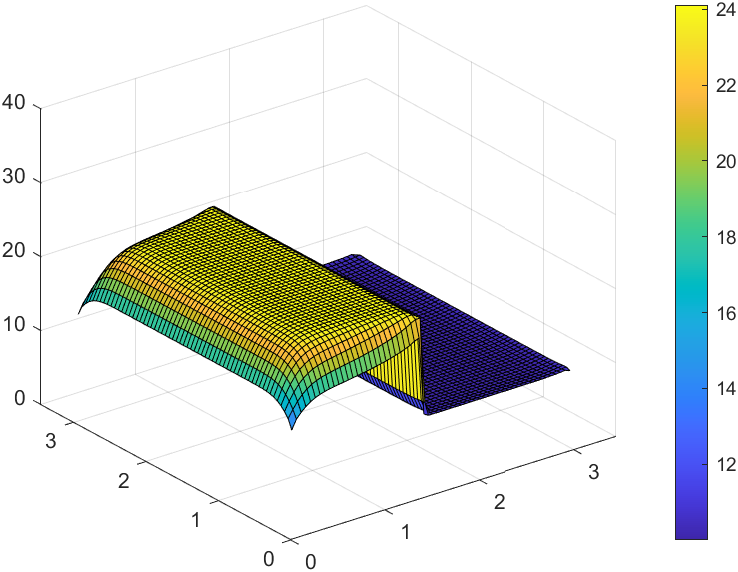
\includegraphics[width = 5.5cm]{figures/Nextroom-start.png}
    }\qquad
    \subfigure[空调向上扫风]{
    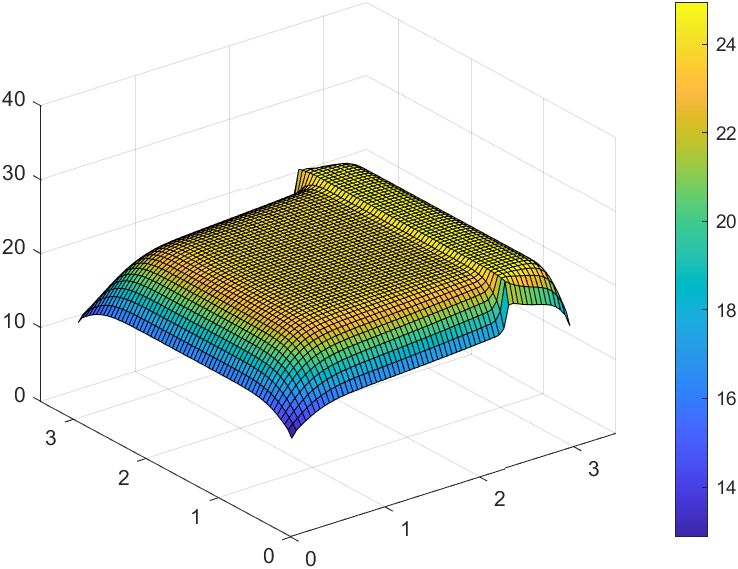
\includegraphics[width = 5.5cm]{figures/Nextroom-up.png}
    }\qquad
    \subfigure[空调向下扫风]{
    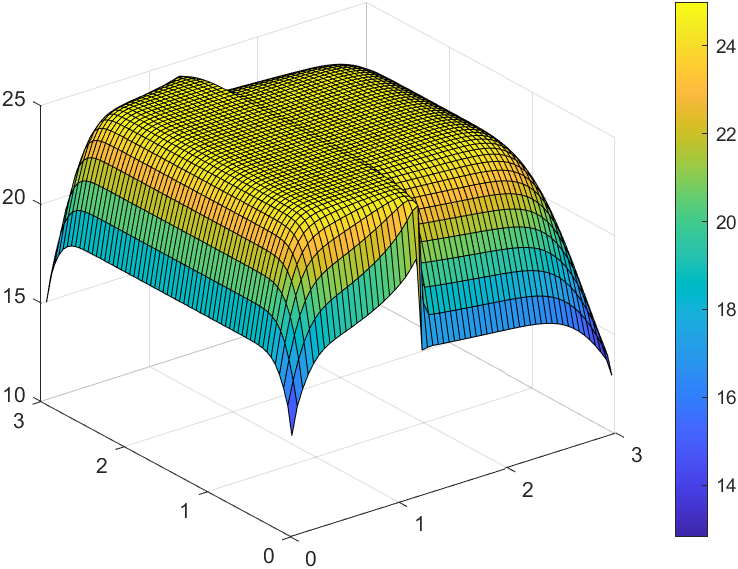
\includegraphics[width = 5.5cm]{figures/Nextroom-down.png}
    }\qquad
    \subfigure[房间竖直截面温度分布图]{
    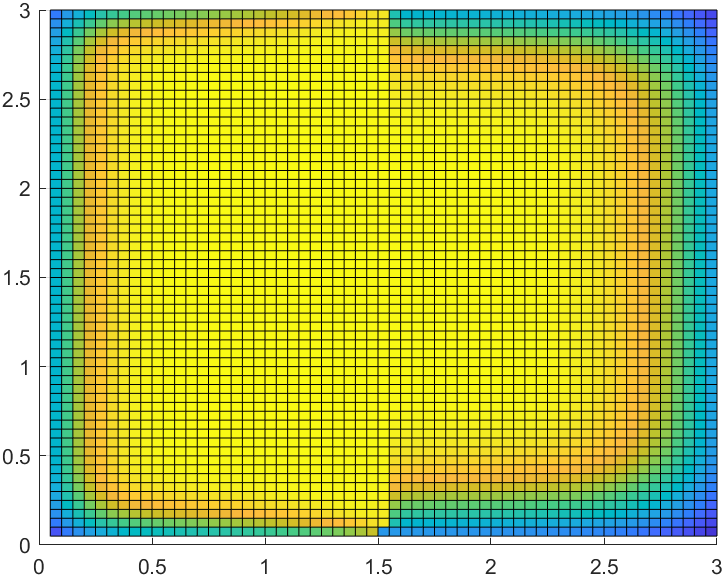
\includegraphics[width = 5.5cm]{figures/nextroom 2d.png}
    }\qquad
    
    \caption{隔壁房间开暖气时的温度分布}
    \label{隔壁房间开暖气时的温度分布}
\end{figure}


可以得到设置25℃空调时,室内的平均温度为23℃,墙边的平均温度为18℃。因此在研究待测房间的传热过程时将18℃作为边界条件。



\subsection{地暖}

将地暖简化为第二类边界条件,即:
\begin{equation}
    -k\frac{\partial T}{\partial x}\big|_{x=L} = q
\end{equation}

式中q为地暖单位面积的放热量,为了方便计算,将上式写作:
\begin{equation}
    T_{x+dx} = T_x -\frac{q}{k}dx
\end{equation}

房间内温度分布如下图所示:
\begin{figure}[h]
    \centering
    \subfigure[主视图]{
    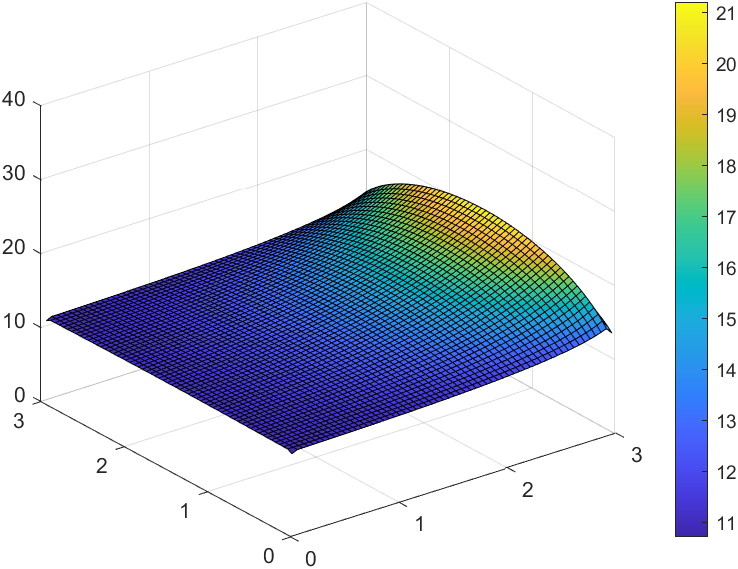
\includegraphics[width = 5.5cm]{figures/地暖主视.png}
    }\qquad
    \subfigure[俯视图]{
    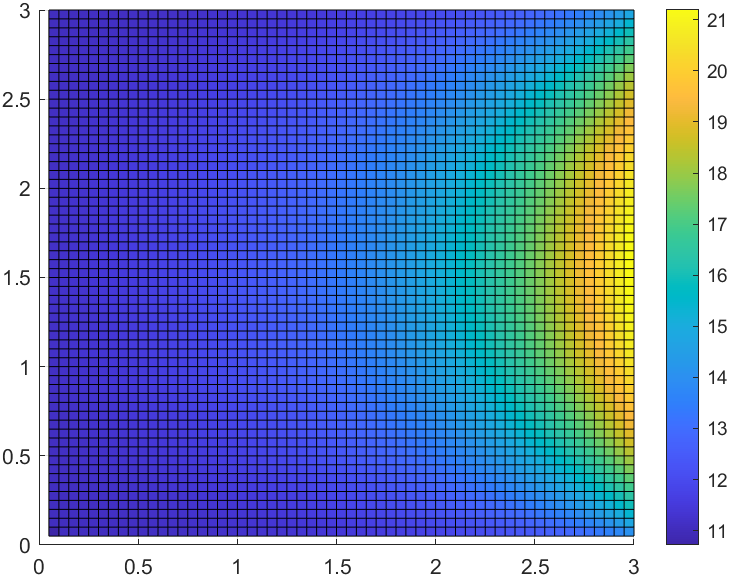
\includegraphics[width = 5.5cm]{figures/地暖俯视.png}
    }
    \caption{隔壁房间开地暖时的温度分布}
    \label{fig:dinuan}
\end{figure}

房间的平均温度为14℃,但是靠近地暖部分的温度较高。出现该现象的原因是地暖模型被过度简化,与现实中的地暖功能产生较大的偏差。因此还是使用开暖气时的隔壁房间平均温度作为待测房间的边界条件,同时考虑待测房间楼上开地暖时对于待测房间温度分布的影响。

\subsection{冷气}

冷气与暖气一样可以简化为一个以匀速在空间内上下移动的恒温热源,热源温度低于环境温度。当外界温度及室内初始物温度为35℃,室内温度设定为25度时,通过\eqref{final equation}可以得出随时间变化的房间温度分布。

房间内某几个时刻的温度分布如图\eqref{隔壁房间开冷气时的温度分布}所示。
\\
\begin{figure}[h]
    \centering
    \subfigure[空调刚开启时]{
    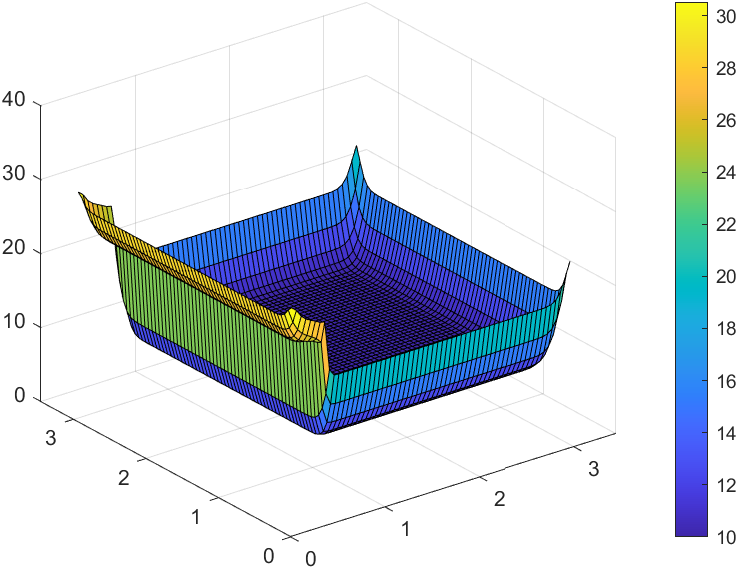
\includegraphics[width = 5.5cm]{figures/nr-cold-start.png}
    }\qquad
    \subfigure[空调向上扫风]{
    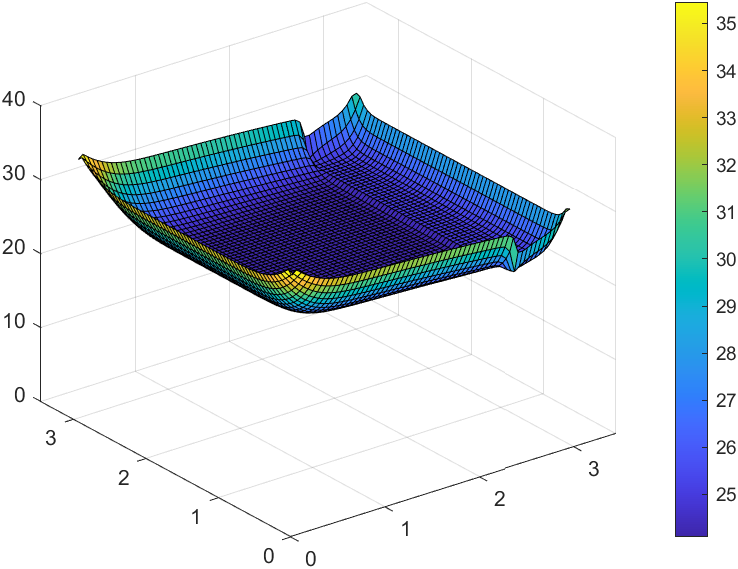
\includegraphics[width = 5.5cm]{figures/nr-cold-up.png}
    }\qquad
    \subfigure[空调向下扫风]{
    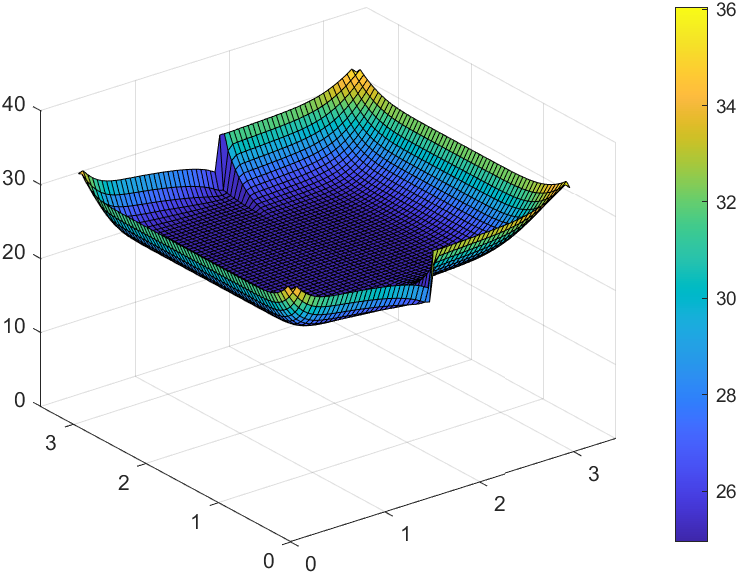
\includegraphics[width = 5.5cm]{figures/nr-cold-down.png}
    }\qquad
    \subfigure[房间竖直截面温度分布图]{
    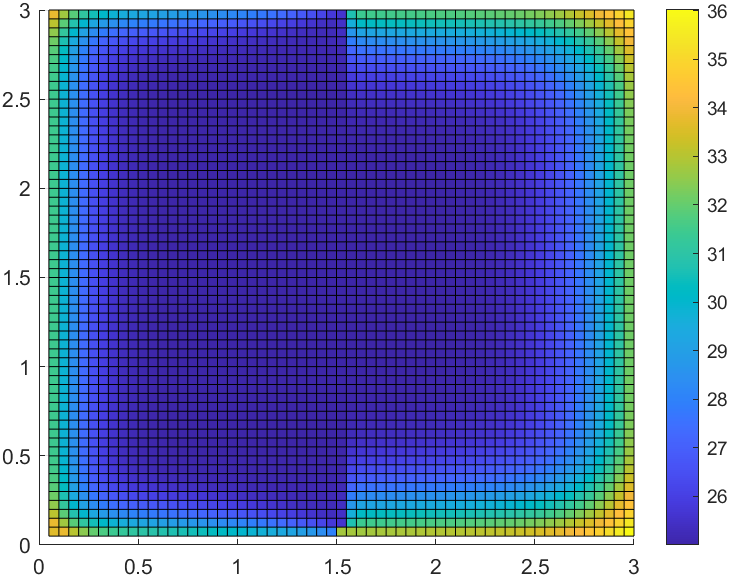
\includegraphics[width = 5.5cm]{figures/nr-cold-2d.png}
    }\qquad
    
    \caption{隔壁房间开冷气时的温度分布}
    \label{隔壁房间开冷气时的温度分布}
\end{figure}

可以得到设置25℃空调时,室内的平均温度为26.8℃,墙边的平均温度为31℃。因此在研究待测房间的传热过程时将31℃作为边界条件。


\newpage

\section{非采暖房间温度估算}

对待测房间,设置其上下左右房间都开启暖气/空调,由于下方以及左右房间地暖开启对待测房间影响不大,因此只考虑上方房间的地暖。即房间的边界条件为:
\begin{equation}
    \begin{cases}
    -k\frac{\partial \boldsymbol{T}}{\partial x}\big|_{x=0} = q'' \\
    \boldsymbol{T}(:,0,t) = T_{next} \\
    \boldsymbol{T}(:,L_y,t) = T_{next} \\
    \boldsymbol{T}(L_x,:,t) = T_{next}
    \end{cases}
    \label{boundary}
\end{equation}

\subsection{冬天}

将$T_{next}=18℃$代入上式,并使用Matlab进行仿真。房间温度分布如下图所示:
\\
\begin{figure}[h]
    \centering
    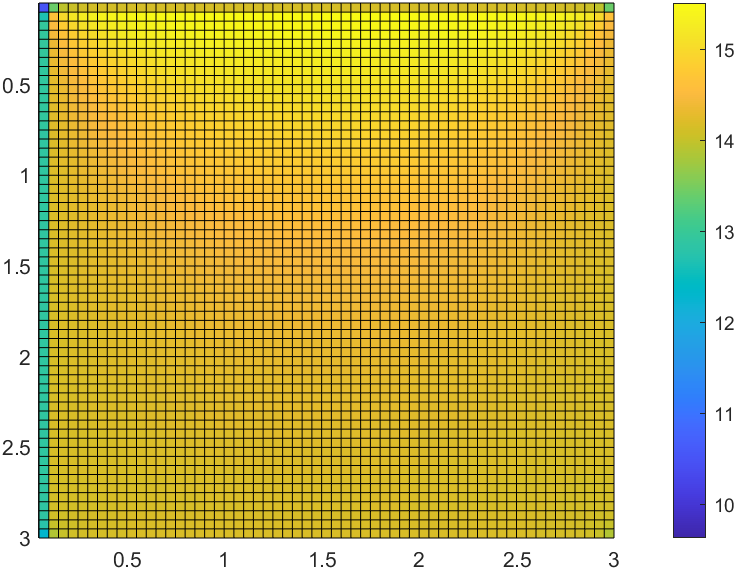
\includegraphics[width = 5.5cm]{figures/mainroom-winter.png}
    \caption{冬天非采暖房间温度分布}
    \label{冬天非采暖房间温度分布l}
\end{figure}
冬天非采暖房间的平均温度为14.4℃

\subsection{夏天}

夏天时忽略上方房间地暖的影响,同时将$T_next = 26.8℃$代入\eqref{boundary},使用Matlab进行仿真,房间的温度分布如下图所示:
\\
\begin{figure}[h]
    \centering
    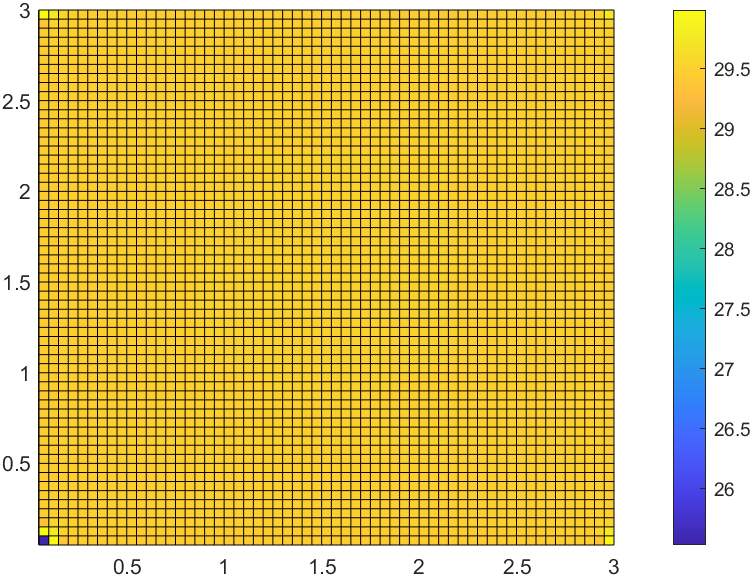
\includegraphics[width = 5.5cm]{figures/mainroom-summer.png}
    \caption{夏天非采暖房间温度分布}
    \label{夏天非采暖房间温度分布}
\end{figure}

夏天非采暖房间的平均温度为29℃。

在进行仿真时,由于夏天房间墙壁上的热流方向与冬天房间墙壁相反,因此需要调整室内传热和墙壁导热的计算顺序,否则会出现结果不准确的现象。

综上所述,可知在冬天或夏天时,隔壁房间打开空调会对所处房间的温度分布有着较为明显的影响,经计算,平均能够节约$20\%$的电费。但是本文的计算结果并不精确,原因有以下几点:
\begin{itemize}
    \item 房间的物理模型过于简化,无论是房间的尺寸还是承重墙的参数,亦或是空调和地暖的布局都过于艰难,无法对真实的户型的温度分布提供参考
    \item 传热过程过于简化,本文仅仅将空调和地暖分别简化为了第一类边界条件和第二类边界条件,事实上在分析开暖气/冷气的房间温度分布时还需要考虑对流传热的影响;以及直接将隔壁房间的平均温度作为待测房间的边界条件也过于草率。
    \item 本文在编写代码时为了避免出现不收敛的结果,对许多物理参数进行了调整,在时间上出现了较大的失真
\end{itemize}

但是本文分析所得的结果仍然能够对非采暖房间的温度分布估算提供定性的参考,为了进一步完善模型,接下来对其他影响待测房间温度分布的因素进行分析。

\section{其他影响因素}

其他影响因素主要考虑房间的窗户和墙壁设置。根据傅里叶定律,墙体对房间温度的影响主要与墙体的厚度以及导热系数有关。一般而言,承重墙、非承重墙以及楼板的厚度都有所不同,会影响隔壁房间对待测房间的温度影响。在考虑开启空调和地暖的情况下,选择导热系数低的墙体材料,例如硬泡聚氨酯复合板、硬泡聚氨酯陶瓷等都有助于增加墙壁的保温隔热性能,减少能量的消耗。

除此以外,墙壁外立面的颜色等也会影响室内温度。以黑色外立面的墙壁为例,在夏天环境温度为32℃时,墙体的温度较一般墙体上升了5℃,对室内的制冷造成了一定的负担。但同时这一类墙体在冬天也能为室内的采暖减轻负担。

在考虑建筑结构上出现承重墙与非承重墙的时候,墙体结构也会对导热产生影响。部分非承重墙为了节省建筑材料会采用中空的结构。由于空气的导热系数远小于墙体材料的导热系数,因此该类非承重墙能够提升室内的保温效果。非承重墙往往用于隔离出卫生间、厨房等区域,这类区域在使用时往往会产生大量的热量,例如在卫生间内淋浴、在厨房内烧菜。因此采用中空结构的非承重墙能够在冬天很好地保持这些区域的温度,提高居住的舒适度。

除了墙体以外,窗户的结构也对室内温度有着显著的影响。首先从结构上而言,目前大范围使用的双层玻璃有着与中空非承重墙一样的传热学原理,能够增强窗户的隔热效果。同时也出现了类似于三层中空玻璃的结构,亦或是向玻璃的中空层中填充氩气等惰性气体,这些设计都提升玻璃的隔热效果,减少室内制冷或采暖时的能量消耗。

同时窗户的面积也对室内温度有着显著的影响,但是由于不同户型的墙面面积不同,单纯比较窗户的面积没有任何参考的价值,因此引入窗墙比的概念。因为玻璃的传热系数大于墙体,因此窗墙比越大的建筑,采暖时的能量损耗也越大。《公共建筑节能设计标准》GB50189-2005第4.2.4条规定:建筑每个朝向的窗(包括透明幕墙)墙面积比均不应大于0.70。当窗(包括透明幕墙)墙面积比小于0.40时,玻璃(或其他透明材料)的可见光透射比不应小于0.40。但是当下人们对于建筑的审美往往要求房间能够有较大的窗墙比,从而获得更好的采光并且能让房间看上去更加通透,更加适合居住。因此设计出隔热性能更好的透明窗户方案抑或是可随户主意愿调节采光度的非透明玻璃幕墙都不失为有前景的研究方向。


\begin{thebibliography}{99}  
\bibitem{ref1}李镒如. 家用空调器供暖对室内热环境影响研究[D].哈尔滨工业大学,2021.
\bibitem{ref2}范征宇,肖子一,刘加平.多气候区不同窗墙比下功能布局对办公建筑能耗的影响[J].建筑节能(中英文),2023,51(06):18-23+31.
\end{thebibliography}

\newpage
\begin{appendices}
    \section{附录:估算隔壁房间温度时使用的代码}

    \begin{lstlisting}[language = matlab]
    clear;
    clc;

    % 设置房间参数
    Lx = 3;
    Ly = 3;
    Lwall = 0.2;
    time = 1;

    % 设置空间步长和时间步长
    dx = 0.05;
    dy = 0.05;
    dt = 0.0001;

    % 矩阵设置
    x = 0:dx:Lx+2*Lwall+0.05;
    y = 0:dy:Ly+2*Lwall+0.05;
    t = 0:dt:time;
    wall = 0:dx:Lwall;

    lengthx = Lx/dx;
    lengthy = Ly/dy;

    %设置系数矩阵
    Ax = (-2*eye(lengthx)+diag(ones(1,lengthx-1),1) + diag(ones(1,lengthx-1),-1));
    Ay = (-2*eye(lengthy)+diag(ones(1,lengthy-1),1) + diag(ones(1,lengthy-1),-1));

    % 设置初始条件
    t0 = 10;    % 初始室温
    T0 = t0*ones(length(x),length(y));


    % 设置边界条件
    top = 10; % 第一类边界条件,开空调
    bottom = 10;
    left = 10;
    right = 10;

    alpha = 2.26;   % 空气热扩散系数
    Tset = 25;

    % 考虑开空调情况下的房间温度
    T = T0;

    q2 = 9;

    % 设置室内温度
    indoor = T(length(wall):length(x)-length(wall)-1,length(wall)+1:length(y)-length(wall));
    indoor_before = indoor;

    indoorx = 0.05:dx:Lx;
    indoory = 0.05:dy:Ly;

    % 生成网格采样点
    [Y,X] = meshgrid(indoory,indoorx);

    i = 1;
    k = 1;

    for n = 1:length(t)-1

        % 边界条件
        T(:,1) = left;
        T(:,length(x)) = right;
        T(1,:) = top;
        T(length(y),:) = bottom;
        
        % 热源

        % 空调扫风
    %     if mod(n,3) == 1
    %         if (i < lengthx) && (i > 1) 
    %             i = i + k;        
    %         else
    %             k = -k;
    %             i = i + k;
    %         end
    %     end
    % 
    %     if i == 0 
    %        i = 1;
    %     end
    %     
    %     indoor(i,:) = Tset;
        
        % 地暖
        indoor(lengthx,:) = indoor_before(lengthx - 1,:) + q2*dx;


        % 室内热传导
        indoor = indoor + alpha*(1/dx^2*Ax*indoor + 1/dy^2*indoor*Ay)*dt;

        % 墙壁隔热
        q = (left - indoor(:,1))/Lwall;
        indoor(:,1) = indoor_before(:,2) + q*dx;

        q = (right - indoor(:,lengthx))/Lwall;
        indoor(:,lengthx) = indoor_before(:,lengthx-1) + q*dx;

        q = (bottom - indoor(lengthy,:))/Lwall;
        indoor(lengthy,:) = indoor_before(lengthy-1,:) + q*dx;

        q = (top - indoor(1,:))/Lwall ;
        indoor(1,:) = indoor_before(2,:) + q*dx;


        indoor_before = indoor;

        T(length(wall):length(x)-length(wall)-1,length(wall)+1:length(y)-length(wall)) = indoor;

        % 生成实时图像
    %     surf(X,Y,indoor)
    %     axis([x(1) x(end) y(1) y(end) 0 40])
    %     getframe;
        
    end
        
        surf(X,Y,indoor)
        axis([x(1) indoorx(end) y(1) indoory(end) 0 40])
\end{lstlisting}

        
    \section{附录:估算非采暖房间温度时使用的代码}

    \begin{lstlisting}[language = matlab]
clear;
clc;

% 设置房间参数
Lx = 3;
Ly = 3;
Lwall = 0.2;
time = 1;

% 设置空间步长和时间步长
dx = 0.05;
dy = 0.05;
dt = 0.0001;

% 矩阵设置
x = 0:dx:Lx+2*Lwall+0.05;
y = 0:dy:Ly+2*Lwall+0.05;
t = 0:dt:time;
wall = 0:dx:Lwall;

lengthx = Lx/dx;
lengthy = Ly/dy;

%设置系数矩阵
Ax = (-2*eye(lengthx)+diag(ones(1,lengthx-1),1) + diag(ones(1,lengthx-1),-1));
Ay = (-2*eye(lengthy)+diag(ones(1,lengthy-1),1) + diag(ones(1,lengthy-1),-1));



% 设置初始条件
t0 = 10;    % 初始室温
T0 = t0*ones(length(x),length(y));

% 冬天
% 设置边界条件
top = 18; % 第一类边界条件,开空调
bottom = 18;
left = 18;
right = 18;

alpha = 2.26;   % 空气热扩散系数

T = T0;
% 设置室内温度
indoor = T(length(wall):length(x)-length(wall)-1,length(wall)+1:length(y)-length(wall));
indoor_before = indoor;
indoorx = 0.05:dx:Lx;
indoory = 0.05:dy:Ly;

% 生成网格采样点
[Y,X] = meshgrid(indoory,indoorx);

for n = 1:length(t)-1

    % 边界条件
    T(:,1) = left;
    T(:,length(x)) = right;
    T(1,:) = top;
    T(length(y),:) = bottom;

    % 冬天
    % 墙壁隔热
    q = (left - indoor(:,1))/Lwall;
    indoor(:,1) = indoor_before(:,1) + q*dx;

    q = (right - indoor(:,lengthx))/Lwall;
    indoor(:,lengthx) = indoor_before(:,lengthx) + q*dx;

    q = (bottom - indoor(lengthy,:))/Lwall;
    indoor(lengthy,:) = indoor_before(lengthy,:) + q*dx;

     q = (top - indoor(1,:))/Lwall ;
    indoor(1,:) = indoor_before(1,:) + q*dx;

   
    % 室内热传导
    indoor = indoor + alpha*(1/dx^2*Ax*indoor + 1/dy^2*indoor*Ay)*dt;


    % 夏天
    % 室内热传导
%     indoor = indoor + alpha*(1/dx^2*Ax*indoor + 1/dy^2*indoor*Ay)*dt;
% 
%     % 墙壁隔热
%     q = (left - indoor(:,1))/Lwall;
%     indoor(:,1) = indoor_before(:,1) + q*dx;
% 
%     q = (right - indoor(:,lengthx))/Lwall;
%     indoor(:,lengthx) = indoor_before(:,lengthx) + q*dx;
% 
%     q = (bottom - indoor(lengthy,:))/Lwall;
%     indoor(lengthy,:) = indoor_before(lengthy,:) + q*dx;
% 
%      q = (top - indoor(1,:))/Lwall+q2;
%     indoor(1,:) = indoor_before(1,:) + q*dx;
% 
% 
%     indoor_before = indoor;
% 
%     T(length(wall):length(x)-length(wall)-1,length(wall)+1:length(y)-length(wall)) = indoor;


    indoor_before = indoor;

    T(length(wall):length(x)-length(wall)-1,length(wall)+1:length(y)-length(wall)) = indoor;

    % 生成实时图像
    surf(X,Y,indoor)
    axis([x(1) x(end) y(1) y(end) 0 40])
    getframe;
     
end
    
    surf(X,Y,T)
    axis([indoorx(1) indoorx(end) indoory(1) indoory(end) 0 40])


\end{lstlisting}
\end{appendices}


\end{document}